 \newpage

\subsubsection{XGBoost}
\label{sec:xgboost}

As discussed earlier, the XGBoost classifier was first trained with default parameters across a range of subsets of data before attempting to optimise parameters using 10 Fold Stratified Cross Validation to verify results across the training set. Finally, the test set (30\% of the overall data) was used to evaluate each model on a series of unseen data.

In the initial experiments, even without tuning parameters, the models achieved a high performance across all metrics. Table \ref{tab:xgb-scv-metrics} summarises the average metrics with 10 Fold Stratified Cross-Validation and Table \ref{tab:xgb-test-metrics} shows the metrics across the 30\% test set. Due to the numerous models created during experimentation, only the most notable models are included in the tables.


\begin{table}[h]
\centering
\caption{XGBoost S-CV Metrics}
\label{tab:xgb-scv-metrics}
\begin{tabular}{|l|l|l|l|l|l|l|l|}
\hline
\textbf{Model ID} & \textbf{Dataset} & \textbf{AUC} & \textbf{F1} & \textbf{Precision} & \textbf{Recall} & \textbf{Accuracy}  \\ \hline
1006 & 100\% & 99.99 & 99.64 & 99.64 & 99.64 & 99.64 \\ \hline
1008 & 100\% & 99.99 & 99.64 & 99.64 & 99.65 & 99.65 \\ \hline
1010 & 100\% & 100.00 & 99.65 & 99.65 & 99.66 & 99.66 \\ \hline
1011 & 100\% & 100.00 & 99.64 & 99.64 & 99.65 & 99.65 \\ \hline
\end{tabular}
\end{table}



\begin{table}[h]
\centering
\caption{XGBoost Test Metrics}
\label{tab:xgb-test-metrics}
\begin{tabular}{|l|l|l|l|l|l|l|l|}
\hline
\textbf{Model ID} & \textbf{Dataset} & \textbf{AUC} & \textbf{F1} & \textbf{Precision} & \textbf{Recall} & \textbf{Accuracy}  \\ \hline
1000 & 60\% & 99.99 & 99.63 & 99.64 & 99.64 & 99.64 \\ \hline
1001 & 80\% & 99.99 & 99.64 & 99.65 & 99.65 & 99.65 \\ \hline
1002 & 80\% & 99.99 & 99.64 & 99.64 & 99.64 & 99.64 \\ \hline
1003 & 80\% & 99.99 & 99.64 & 99.64 & 99.64 & 99.64 \\ \hline
1005 & 80\% & 99.99 & 99.64 & 99.65 & 99.65 & 99.65 \\ \hline
1006 & 100\% & 99.99 & 99.65 & 99.65 & 99.65 & 99.65 \\ \hline
1008 & 100\% & 99.99 & 99.65 & 99.65 & 99.65 & 99.65 \\ \hline
1010 & 100\% & 99.99 & 99.65 & 99.65 & 99.66 & 99.66 \\ \hline
1011 & 100\% & 99.99 & 99.65 & 99.65 & 99.65 & 99.65 \\ \hline
\end{tabular}
\end{table}


%\begin{table}[h]
%\centering
%\caption{XGB Model Metrics}
%\label{tab:xgb-metrics}
%\begin{tabular}{|l|l|l|l|l|l|l|l|}
%\hline
%\textbf{Model} & \textbf{Device} & \textbf{Dataset} & \textbf{AUC} & \textbf{Accuracy} & \textbf{Precision} & \textbf{Recall} & \textbf{F1}  \\ \hline
%Base & M2 & 80\% & ? & 99.7 & 95.5 & 88.2 & 91.5 \\ \hline
%Base & M2 & 100\% & ? & ? & ? & ? & ? \\ \hline
%Base & VM & 60\% & ? & 99.6 & 95.0 & 88.4 & 91.4 \\ \hline
%Base & VM & 80\% & 1.00 & 99.6 & 94.9 & 87.8 & 91.0 \\ \hline
%Base & VM & 100\% & ? & 99.7 & 99.7 & 99.7 & 99.6 \\ \hline
%Optimised & VM & 80\% & 1.00 & 99.6 & 99.6 & 99.6 & 99.6 \\ \hline
%Optimised & VM & 100\% & 1.00 & 99.7 & 99.6 & 99.7 & 99.6 \\ \hline
%RGS & VM & 100\% & 99.99 & 99.66 & 99.65 & 99.66 & 99.65 \\ \hline
%\end{tabular}
%\end{table}

\subsubsection*{Randomised GridSearch}

An attempt was made to utilise GridSearchCV for parameter optimization; significant setbacks were encountered in achieving a successful execution due to numerous errors, system crashes, and exceptionally high grid search time. In light of the difficulties faced with GridSearchCV, RandomizedSearchCV was utilised instead, This decision was justified by several factors:

RandomizedSearchCV uses a subset of parameter combinations sampled from a defined grid. This approach heavily reduces the computational power required compared to the exhaustive search needed for GridSearchCV. Moreover, RandomizedSearchCV enables striking a balance between computational resources and search comprehensiveness by defining the number of iterations to evaluate. See Listing \ref{lst:param_grid_xgb} for the parameter grid used.

\medskip

\begin{lstlisting}[language=Python, caption={Grid Search Parameters For XGBoost}, label= lst:param_grid_xgb]
param_grid = {
    'learning_rate': [0.01, 0.1, 0.3],
    'max_depth': [3, 6, 9],
    'min_child_weight': [1, 3, 5],
    'gamma': [0, 0.1, 0.2],
    'subsample': [0.5, 0.7, 0.9],
    'colsample_bytree': [0.5, 0.7, 0.9],
    'n_estimators': [100, 200]
}
\end{lstlisting}

\textbf{Best Found Parameters}
\medskip

Using the best-found parameters from the RandomizedSearchCV, a new model was created, referenced above as ID 1010. Table \ref{tab:xg_rgs_parameters} highlights the optimal parameters found.

\begin{table}[h]
\captionsetup{justification=centering} 
\centering
\caption{XGBoost RGS Parameters}
\begin{tabular}{ll}
\hline
\textbf{Parameter} & \textbf{Value} \\ \hline
Early Stopping & 10 \\
Evaluation Metric & merror \\
Learning Rate & 0.3 \\
Max Depth & 9 \\
Min Child Weight & 3 \\
Gamma & 0 \\
Subsamples & 0.9 \\
Colsample By Tree & 0.7 \\
N Estimators & 200 \\ \hline
\end{tabular}
\label{tab:xg_rgs_parameters}
\end{table}


\textbf{Optimised Model}
\medskip

A new model was created with the best-found parameters, this is referred to as the 'Optimised Model'/(ID 1010) in this section. The model performed very well, with an average AUC of 99.99 on the training data and 99.98 on the test data. The F1 score is 99.65 on the test set indicating the model has a high proportion of correct predictions, balancing both precision and recall well. The confusion matrix verifies this and shows the model to perform well for most classes, especially Normal, SDDP and Web Spoofing with almost perfect precision and recall. However, there are a few misclassifications for 'Botnet', 'Malware' and 'SSH'. The model struggled and occasionally misclassified Normal traffic as malicious, but performed well in the SQL Injection class, especially given the small number of samples. The Cross-validation and test set results are similar and indicate the model is not overfitting and generalising well to new data. Refer to \ref{fig:xgb_optimised_fi}, \ref{fig:xgb_optimised_cm} and \ref{tab:optimised_xgboost} for metrics.

Using the total number of instances of each class, the misclassification report can be calculated for each and is shown accordingly:

\begin{itemize}
	\item Botnet: 4208 / 17060 = {\color{red} 25\%}
	\item Malware: 7161 / 39476 = 18\%
	\item Normal: 6365 / 4572206 = 0.0013\%
	\item SQL: 89 / 789 = 11\%
	\item SSDP: 0 / 1649955 = {\color{mygreen} 0\%}
	\item SSH: 771 / 3565 = 21\%
	\item WebSpoof: 3046 / 121533 = 2.5\%
\end{itemize}


\begin{figure}[H]
\centering
\caption{Optimised XGBoost Model FI}
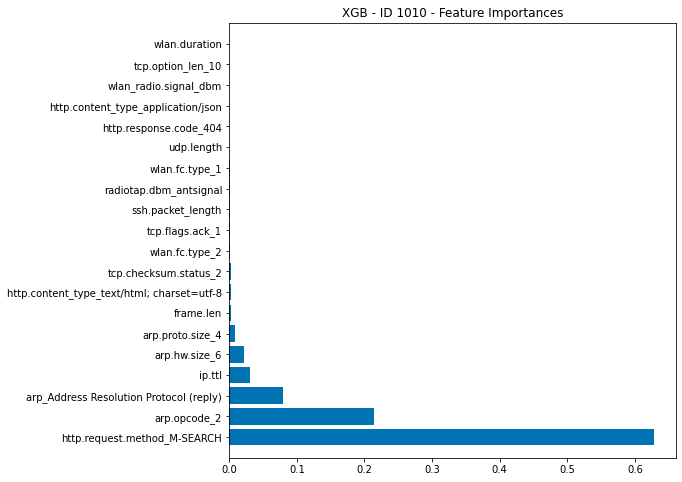
\includegraphics[width=\textwidth]{Appendices/Images/XGB/xgb_1010_fi.png}
\label{fig:xgb_optimised_fi}
\end{figure}

\clearpage
\begin{table}[hp]
  \centering
  \caption{Optimised XGBoost Classification Report}
  \label{tab:optimised_xgboost}
    \begin{tabular}{lcccc}
    \toprule
    Class & Precision & Recall & F1-Score & Support \\
    \midrule
    Botnet & 0.96 & {\color{red}\bfseries 0.75} & {\color{red}\bfseries 0.84} & 17060 \\
    Malware & {\color{red}\bfseries 0.89} & 0.82 & 0.85 & 39476 \\
    Normal & 1.00 & 1.00 & 1.00 & 4572206 \\
    SQL Injection & 0.94 & 0.89 & 0.91 & 789 \\
    SSDP & 1.00 & 1.00 & 1.00 & 1649955 \\
    SSH & 0.92 & 0.78 & 0.85 & 3565 \\
    Website Spoofing & 0.99 & 0.97 & 0.98 & 121533 \\
    \midrule
    Accuracy & & & 1.00 & 6404584 \\
    Macro Avg & 0.96 & 0.89 & 0.92 & 6404584 \\
    Weighted Avg & 1.00 & 1.00 & 1.00 & 6404584 \\
    \bottomrule
    \end{tabular}
\end{table}

\begin{figure}[H]
\centering
\caption{Optimised XGBoost Model CM}
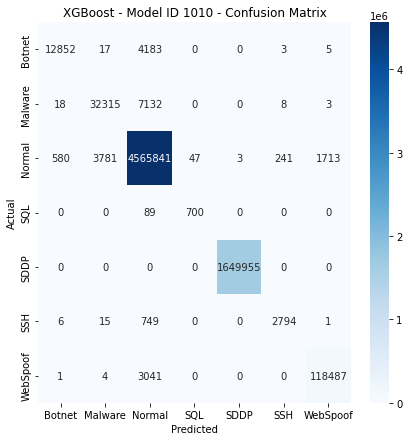
\includegraphics[width=0.9\textwidth]{Appendices/Images/XGB/xgb_1010_cm.png}
\label{fig:xgb_optimised_cm}
\end{figure}



%
%\begin{table}[h]
%\centering
%\caption{XGBoost Evaluation Metrics}
%\label{tab:xgb-eval-metrics}
%\begin{tabular}{|l|l|l|l|l|l|l|l|}
%\hline
%\textbf{Model} & \textbf{Device} & \textbf{Size} & \textbf{AUC} & \textbf{F1} & \textbf{Precision} & \textbf{Recall} & \textbf{Accuracy} \\ \hline
%Stock & M2 & 80\% & ? & 91.5 & 95.5 & 88.2 & 99.7 \\ \hline
%Stock & M2 & 100\% & 99.99 & 99.65 & 99.65 & 99.65 & 99.65 \\ \hline
%Stock & VM & 60\% & ? & 91.4 & 95.0 & 88.4 & 99.6 \\ \hline
%Stock & VM & 80\% & 1.00 & 91.0 & 94.9 & 87.8 & 99.6 \\ \hline
%Stock & VM & 100\% & ? & 99.6 & 99.7 & 99.7 & 99.7 \\ \hline
%Optimised & VM & 80\% & 1.00 & 99.6 & 99.6 & 99.6 & 99.6 \\ \hline
%Optimised & VM & 100\% & 1.00 & 99.6 & 99.6 & 99.7 & 99.7 \\ \hline
%RGS & VM & 100\% & 99.99 & 99.65 & 99.65 & 99.66 & 99.66 \\ \hline
%\end{tabular}
%\end{table}

